% \subsection{Optimize Stage-in Phase}
% In the stage-in phase, only burst buffer demand is considered.
% Scheduling is made based on the value of $bb\_in$ of jobs in $Q_I$.
% If we care about data transfer throughput,
% we should transfer as much data as possible by doing the following optimization:
% \begin{align*}
%         & \max \sum_{i\in S} bb\_in_i \\
%         & s.t. \sum_{i\in S} bb\_in_i \leq BB_{available} \numberthis \label{Equ:MaxTransferData}
%         %\left\{
%                 %\begin{array}{l}
%                         %S \subseteq J_{Q_I} \\ [1em]
%                         %\sum_{i\in S} bb\_in_i \leq BB_{available}
%                 %\end{array} 
%         %\right.
% \end{align*}
% where $J_{Q_I}$ stands for all jobs in input queue at the time considering,
% $S\subseteq J_{Q_I}$ is the set of job selected by Cerberus,
% $bb\_in_i$ is the burst buffer demand of $job_i$,
% $BB_{available}$ is system's available amount of burst buffer.
% 
% Stage-out phase scheduling are made based on the value of $bb\_out$ of jobs in $Q_O$.
% Optimization formula for different purpose are almost the same as
% Equation~\ref{Equ:MaxTransferData},
% except that $bb\_in$ is replaced with $bb\_out$,
% $J_{Q_I}$ is replaced with $J_{Q_O}$, the job set of output queue.


%==============XY====================
\section{Optimization Enhancement}

Cerberus can be further enhanced with different optimizations when making scheduling decision
for jobs waiting in each queue.

\subsection{Scheduling Optimization in Stage-In/Out Phase}

In the stage-in phase, jobs require only for burst buffer.
Cerberus schedule jobs in $Q_I$ based on their burst buffer demand $bb\_in$.
To maximize burst buffer's utilization,
one can schedule jobs according to the following optimization:
\begin{align*}
        \mathbf{Problem} & \text{ } \mathbf{1} \\
        \max &\sum_{i\in J_{Q_I}} bb\_in_i \cdot x_i \\
        s.t. &\left\{
                \begin{array}{l}
                        x_i \in \{0, 1\}, \forall i \in J_{Q_I}\\ [0.8em] \numberthis \label{Equ:MaxTransferData}
                        \sum_{i \in J_{Q_I}} bb\_in_i \cdot x_i \leq BB_{available}
                \end{array}
        \right.
\end{align*}
%\begin{align*}
        %& \max \sum_{i\in S} bb\_in_i \\
        %& s.t. \sum_{i\in S} bb\_in_i \leq BB_{available} \numberthis \label{Equ:MaxTransferData}
        %%\left\{
                %%\begin{array}{l}
                        %%S \subseteq J_{Q_I} \\ [1em]
                        %%\sum_{i\in S} bb\_in_i \leq BB_{available}
                %%\end{array} 
        %%\right.
%\end{align*}
where $J_{Q_I}$ stands for all jobs in input queue,
$\mathcal{J} = \{x_i|x_i = 1, \text{ } \forall i \in J_{Q_I}\}$ is the set of jobs selected by Cerberus,
$bb\_in_i$ is the burst buffer demand of job $job_i$,
$BB_{available}$ is system's currently available amount of burst buffer.

Stage-out phase scheduling are made based on the value of $bb\_out$ of jobs in $Q_O$.
Optimization formula for stage-out phase are almost the same as
Problem 1, except that $bb\_in$ is replaced with $bb\_out$,
$J_{Q_I}$ is replaced with $J_{Q_O}$, the job set of output queue.


% \subsection{Optimize Running Phase}
% Running jobs require not only compute nodes, but burst buffer to ensure performance and correctness.
% Scheduling are accordingly made based on the value of $c$ and $bb\_run$ of jobs in $Q_R$.
% To maximize multiple types of resource's utilization,
% we convert it to the knapsack problem by defining the value of the $job_i$ as
% \begin{equation}
%         v_i = \frac{c_i / CN}{rt_i} \times \frac{bb\_run_i / BB}{rt_i}
%         \label{Equ:DefValue}
% \end{equation}
% where $rt_i$ is the running time of $job_i$, the time it takes up the computing nodes.
% By defining \textit{value} as Equation~\ref{Equ:DefValue},
% we prefer these tasks that claims to take up node resources with short duration.
% Unfortunately, it is difficult to predict $rt_i$ before actually running the job.
% Of course we could use the \textit{expected running time} $ert_i$ specified by user.
% However, by examining the log traces from Argonne National Laboratory (ANL)\cite{JobTrace},
% we found that the variance between $rt_i$ and $ert_i$ is significantly different.
% For now we can just assume $ert_i$ represent $rt_i$ of $job_i$.
% In the future, we could adopt machine learning or data mining ideas
% to predict the running time of a job with demand vector.
% %Notice that then the value of a task is proportional to $c_i*bb_i$.
% The optimizing formula can thus be
% \begin{align*}
%         & \max \sum_{i \in S}\frac{c_i}{ert_i} * \frac{bb\_run_i}{ert_i} \\
%         & s.t. \left\{
%                 \begin{array}{l}
%                         %S \subseteq J_{Q_R} \\ [1em]
%                         \sum_{i \in S} c_i \leq CN_{available} \\ [0.5em]\numberthis \label{Equ:MaxProduct} 
%                         \sum_{i \in S} bb\_run_i \leq BB_{available}
%                 \end{array} 
%         \right.
% \end{align*}
% where $J_{Q_R}$ is the set of jobs in running queue,
% $S\subseteq J_{Q_R}$ stands for jobs selected by scheduler,
% $CN_{available}$ and $BB_{available}$ represent the amount of system's available resources
% (compute nodes and burst buffer nodes) at current moment.



\subsection{Scheduling Optimization in Running Phase}
Running jobs require not only compute nodes, but also likes to utilize burst buffer to enhance performance.
Here we take a more general strategy.
We define the \textbf{profit} of $job_i$ in $Q_R$ as it is using $c$ compute nodes and $bb\_run$ amount of BB
\begin{equation}
        p_i = f(c_i, bb\_run_i, ert_i)
\label{Equ:GeneralProfit}
\end{equation}
where $ert_i$ is the expected running time of $j_i$.
Then the objective is to maximize the total profit of jobs in running queue, formularized as
\begin{align*}
        \mathbf{Problem} & \text{ } \mathbf{2} \\
        \max &\sum_{i \in J_{Q_R}} p_i \cdot x_i \\
        s.t. &\left\{
                \begin{array}{l}
                        x_i \in \{0, 1\}, \forall i \in J_{Q_R} \\ [0.8em]
                        \sum_{i \in J_{Q_R}} c_i \cdot x_i \leq CN_{available} \\ [0.8em]\numberthis \label{Equ:MaxProduct} 
                        \sum_{i \in J_{Q_R}} bb\_run_i \cdot x_i \leq BB_{available}
                \end{array} 
        \right.
\end{align*}
where $J_{Q_R}$ is the set of jobs in running queue,
$\mathcal{J}  = \{x_i|x_i=1, \text{ } \forall i \in J_{Q_R}\}$ stands for jobs selected by scheduler,
$CN_{available}$ and $BB_{available}$ represent the amount of system's currently available resources.

As an example, in this paper we measure the value of a job based on how efficient it utilize its resource:
\begin{equation}
        v_i = \frac{c_i / CN}{ert_i} \times \frac{bb\_run_i / BB}{ert_i}
        \label{Equ:DefValue}
\end{equation}
where efficiency is measured as the ratio of resource demand to expected running time.
Specializing Problem 2 using $v_i$ favors tasks that claim to take up resources with short duration.
%\begin{align*}
        %& \max \sum_{i \in S}\frac{c_i}{ert_i} * \frac{bb\_run_i}{ert_i} \\
        %& s.t. \left\{
                %\begin{array}{l}
                        %%S \subseteq J_{Q_R} \\ [1em]
                        %\sum_{i \in S} c_i \leq CN_{available} \\ [0.5em]\numberthis \label{Equ:MaxProduct} 
                        %\sum_{i \in S} bb\_run_i \leq BB_{available}
                %\end{array} 
        %\right.
%\end{align*}



\subsection{Solving the Optimization Problems}
% It is trivial to show that optimization problem~\ref{Equ:MaxTransferData}
% is equivalent to 0-1 knapsack problem.
% Problem~\ref{Equ:MaxProduct} can be informally treat as 2-dimension 0-1 knapsack problem.
% We expect all of them are NP-hard problems.
% We can solve them with dynamic programming in pseudo polynomial time.
% Applying memorization could also help accelerate the solving process.
% However, we are not interested in the optimal result of
% problem~\ref{Equ:MaxTransferData} and problem~\ref{Equ:MaxProduct}
% but in a combination of jobs that yields the optimal solution,
% which, fortunately, can also be tracked back down
% using the memorizations kept in dynamic programming.

% %The solution to Problem~\ref{Equ:MaxTransferData},
% %Problem~\ref{Equ:MaxTaskNumber} and Problem~\ref{Equ:MaxProduct} are similar.
% First, for Problem~\ref{Equ:MaxTransferData}, the recursive relationship is
% given by Recursion~\ref{Equ:MaxTransferDataRecursion}.
% In~\ref{Equ:MaxTransferDataRecursion}, the memo we keeps during solving is
% the optimal solution for 
% $jobs=(job_1, job_2, \ldots, job_i)$ with $w$ GB of available burst buffer.
% For Problem~\ref{Equ:MaxProduct}, we keep the memo of the optimal solution 
% for $jobs=(job_1, job_2, \ldots, job_i)$
% with $c$ computing nodes and $w$ GB of burst buffer being available.

% Scheduler can obtain an optimal combination of jobs by tracking along the memo.
% Take the problem~\ref{Equ:MaxProduct} problem for example.
% We start from $dp(n, CN, BB)$.
% If $c_n \leq CN$ and $bb\_in_n \leq BB$, $job_n$ should be scheduled if
% $dp(i-1, c, w) \leq dp(i-1, c - c_i, w - bb\_in_i) + c_i bb\_in_i$ and
% recurse with $dp(n - 1, CN - c_i, BB - bb\_in_i)$;
% otherwise, $job_n$ should be skipped and we recurse the process on $dp(n-1, CN, BB)$.
% The time complexity of solving Recursion~\ref{Equ:MaxTransferDataRecursion} is $O(n\times BB)$.
% The time complexity of solving Recursion~\ref{Equ:MaxProductRecursion}
% is $O(n\times CN\times BB)$.

% Notice that $CN$ and $BB$ may be very large integers,
% making the pseudo-polynomial algorithm unsuitable
% to be used online by scheduler.
% In practice, we could reduce the time complexity by allocating resource
% in a coarser granularity.
% For example, jobs usually asks for compute node in the unit of $cn\_unit = 512$ nodes;
% demands for burst buffer nodes on checkpointing and output are
% usually in the unit of $bb\_unit = 1$ TB.
% We can divide both $CN$ and $c_i$ by $cn\_unit$;
% divide both $BB$ and $bb\_run, bb\_out$ by $bb\_unit$.
% It is also possible to reduce the value of $n$, the number of jobs in the queue.
% For example, we can consider only $\frac{1}{\alpha}n$ jobs in the queue.
% This will give us only the partial optimal solution
% in exchange of less computation complexity.

It is trivial to show that optimization problem~\ref{Equ:MaxTransferData}
is equivalent to 0-1 knapsack problem.
Problem~\ref{Equ:MaxProduct} can be informally treat as 2-dimension 0-1 knapsack problem.
We expect all of them to be NP-hard problems.
Dynamic programming is adopted to solve them in pseudo polynomial time.
Applying memorization could also help accelerate the solving process.
In addition, we are not interested in the optimal result of
problem~\ref{Equ:MaxTransferData} and problem~\ref{Equ:MaxProduct}
but in a combination of jobs $\mathcal{J}$ that yields the optimal solution,
which, fortunately, can also be tracked back down
using the memorizations kept during dynamic programming.
How to fill in memo and track back optimal $\mathcal{J}$ are shown in Algorithm~\ref{Alg:MaxBB}
and Algorithm~\ref{Alg:MaxCPU} for Problem~\ref{Equ:MaxTransferData}
and Problem~\ref{Equ:MaxProduct} respectively.
The time complexity of Algorithm~\ref{Alg:MaxBB} is $O(n\times BB)$.
The time complexity of solving Algorithm~\ref{Alg:MaxCPU} is $O(n\times CN\times BB)$.
%For Problem~\ref{Equ:MaxTransferData}, the recursive relationship is
%given by Recursion~\ref{Equ:MaxTransferDataRecursion}.
%For Problem~\ref{Equ:MaxProduct}, the recursive relationship is
%given by Recursion~\ref{Equ:MaxProductRecursion}.
%The time complexity of solving Recursion~\ref{Equ:MaxTransferDataRecursion} is $O(n\times BB)$.
%The time complexity of solving Recursion~\ref{Equ:MaxProductRecursion}
%is $O(n\times CN\times BB)$.

%\begin{strip}
        %\begin{align}
                %dp(i, w) = & 
                %\left\{
                        %\begin{array}{l}
                                %0, \text{ if $i=0$ } \\ [0.4em]
                                %dp(i-1, w), \text{ if $bb\_in_i > w$} \\ [0.4em]
                                %\max \{ dp(i-1, w), dp(i-1, w-bb\_in_i) + bb\_in_i \}, \text{ if $bb\_in_i \leq w$}
                        %\end{array} 
                %\right.
                %\label{Equ:MaxTransferDataRecursion} 
        %\end{align}
%\end{strip}

%\begin{strip}
        %\begin{align}
                %dp(i, c, w) = &
                %\left\{
                        %\begin{array}{l}
                                %0, \text{ if $i=0$ } \\ [0.4em]
                                %dp(i-1, c, w), \text{ if $c_i > c$ or $bb\_run_i > w$} \\ [0.4em]
                                %\max \{ dp(i-1, c, w), dp(i-1, c - c_i, w - bb\_run_i) + v_i \}, \text{ if $c_i \leq c$ and $bb\_run_i \leq w$}
                        %\end{array} 
                %\right.
                %\label{Equ:MaxProductRecursion}
        %\end{align}
%\end{strip}


\algrenewcommand{\algorithmiccomment}[1]{\hskip1em$/*$ #1 $*/$}

\begin{algorithm}[t]
\caption{Maximize Data Transfer of Jobs in $Q_I$ or $Q_O$}
\label{Alg:MaxBB}
\begin{algorithmic}[1]
        \State $\boldsymbol{bb} \gets $ burst buffer demands of $J_Q = (j_1, j_2,\ldots, j_N)$
        \State $\boldsymbol{dp} \gets \boldsymbol{0}_{(N+1) \times (BB+1)}$
        \State $\mathcal{J} \gets \emptyset$\Comment{scheduling result}
        \\
        \Function{FillInMemo}{ }
                \For{$i \gets 1, N$}
                        \For{$w \gets 1, BB$}
                                \If{$w \geq bb_i$}
                                        \State $dp_1 = dp(i-1, w-bb_i)+bb_i$
                                        \State $dp_2 = dp(i-1, w)$
                                        \State $dp(i, w) \gets \max\{dp_1, dp_2\}$
                                \Else
                                        \State $dp(i,w) \gets dp(i-1,w)$
                                \EndIf
                        \EndFor
                \EndFor
                \State \Call{TrackBackJobs}{$N, BB$}
        \EndFunction
        \\
        \Function{TrackBackJobs}{$i, w$}
                \If{$i > 0$}
                        \If{$w \geq bb_i$}
                                \State $dp_1 = dp(i-1, w-bb_i)+bb_i$
                                \State $dp_2 = dp(i-1, w)$
                                \If{$dp_1 \geq dp_2$}
                                        \State $\mathcal{J} = \mathcal{J} \cup j_i$
                                        \State \Call{TrackBackJobs}{$i-1, w-bb_i$}
                                \Else
                                        \State \Call{TrackBackJobs}{$i-1, w$}
                                \EndIf
                        \Else
                                \State \Call{TrackBackJobs}{$i-1, w$}
                        \EndIf
                \EndIf
        \EndFunction
\end{algorithmic}
\end{algorithm}

\begin{algorithm}[t]
\caption{Maximize Profit of Jobs in $Q_R$}
\label{Alg:MaxCPU}
\begin{algorithmic}[1]
        \State $\boldsymbol{bb} \gets $ burst buffer demands of $J_Q = (j_1, j_2,\ldots, j_N)$
        \State $\boldsymbol{cn} \gets $ compute nodes demands of $j \in J_Q$
        \State $\boldsymbol{dp} \gets \boldsymbol{0}_{(N+1) \times (CN) \times (BB+1)}$
        \State $\boldsymbol{v} \gets$ values of $j \in J_Q$
        \State $\mathcal{J} \gets \emptyset$\Comment{scheduling result} 
        \\
        \Function{FillInMemo}{ }
                \For{$i \gets 1, N$}
                        \For{$c \gets 1, CN$} 
                                \For{$w \gets 1, BB$}
                                        \If{$c \geq cpu_i$ and $w \geq bb_i$}
                                                \State $dp_1 = dp(i-1, c-cn_i, w-bb_i)+v_i$
                                                \State $dp_2 = dp(i-1, c, w)$
                                                \State $dp(i, c, w) \gets \max\{dp_1, dp_2\}$
                                        \Else
                                                \State $dp(i,c,w) \gets dp(i-1,c,w)$
                                        \EndIf
                                \EndFor
                        \EndFor
                \EndFor
                \State \Call{TrackBackJobs}{$N, CN, BB$}
        \EndFunction
        \\
        \Function{TrackBackJobs}{$i, c, w$}
                \If{$i > 0$}
                        \If{$c \geq cpu_i$ and $w \geq bb_i$}
                                \State $dp_1 = dp(i-1, c-cn_i, w-bb_i)+v_i$
                                \State $dp_2 = dp(i-1, c, w)$
                                \If{$dp_1 \geq dp_2$}
                                        \State $\mathcal{J} = \mathcal{J} \cup j_i$
                                        \State \Call{TrackBackJobs}{$i-1, c-cpu_i, w-bb_i$}
                                \Else
                                        \State \Call{TrackBackJobs}{$i-1, c, w$}
                                \EndIf
                        \Else
                                \State \Call{TrackBackJobs}{$i-1, c, w$}
                        \EndIf
                \EndIf
        \EndFunction
\end{algorithmic}
\end{algorithm}

% \subsection{Cerberus Simulation}
% \label{Sec:Simulation}
% 
% We develop an event-driven simulator, named \textbf{BBSim},
% to simulate Cerberus scheduling jobs on the burst buffer enabled HPC system.
% Figure~\ref{Fig:JobFSM} illustrates the BBSim flow chart and the event-driven approach in the simulation.
% The \textit{state} of the job changes depending on current status and
% happening \textit{events}, along with triggered \textit{action}.
% For example, when a job $j_i$ is submitted to the system, 
% it enters \textit{Waiting Stage-in} state, 
% waiting to be scheduled in job queue $Q_I$. 
% The scheduler checks $j_i$ resource demand and 
% dispatches it to run when enough resources become available.
% 
% \begin{figure}[!htbp]
% \centering
%         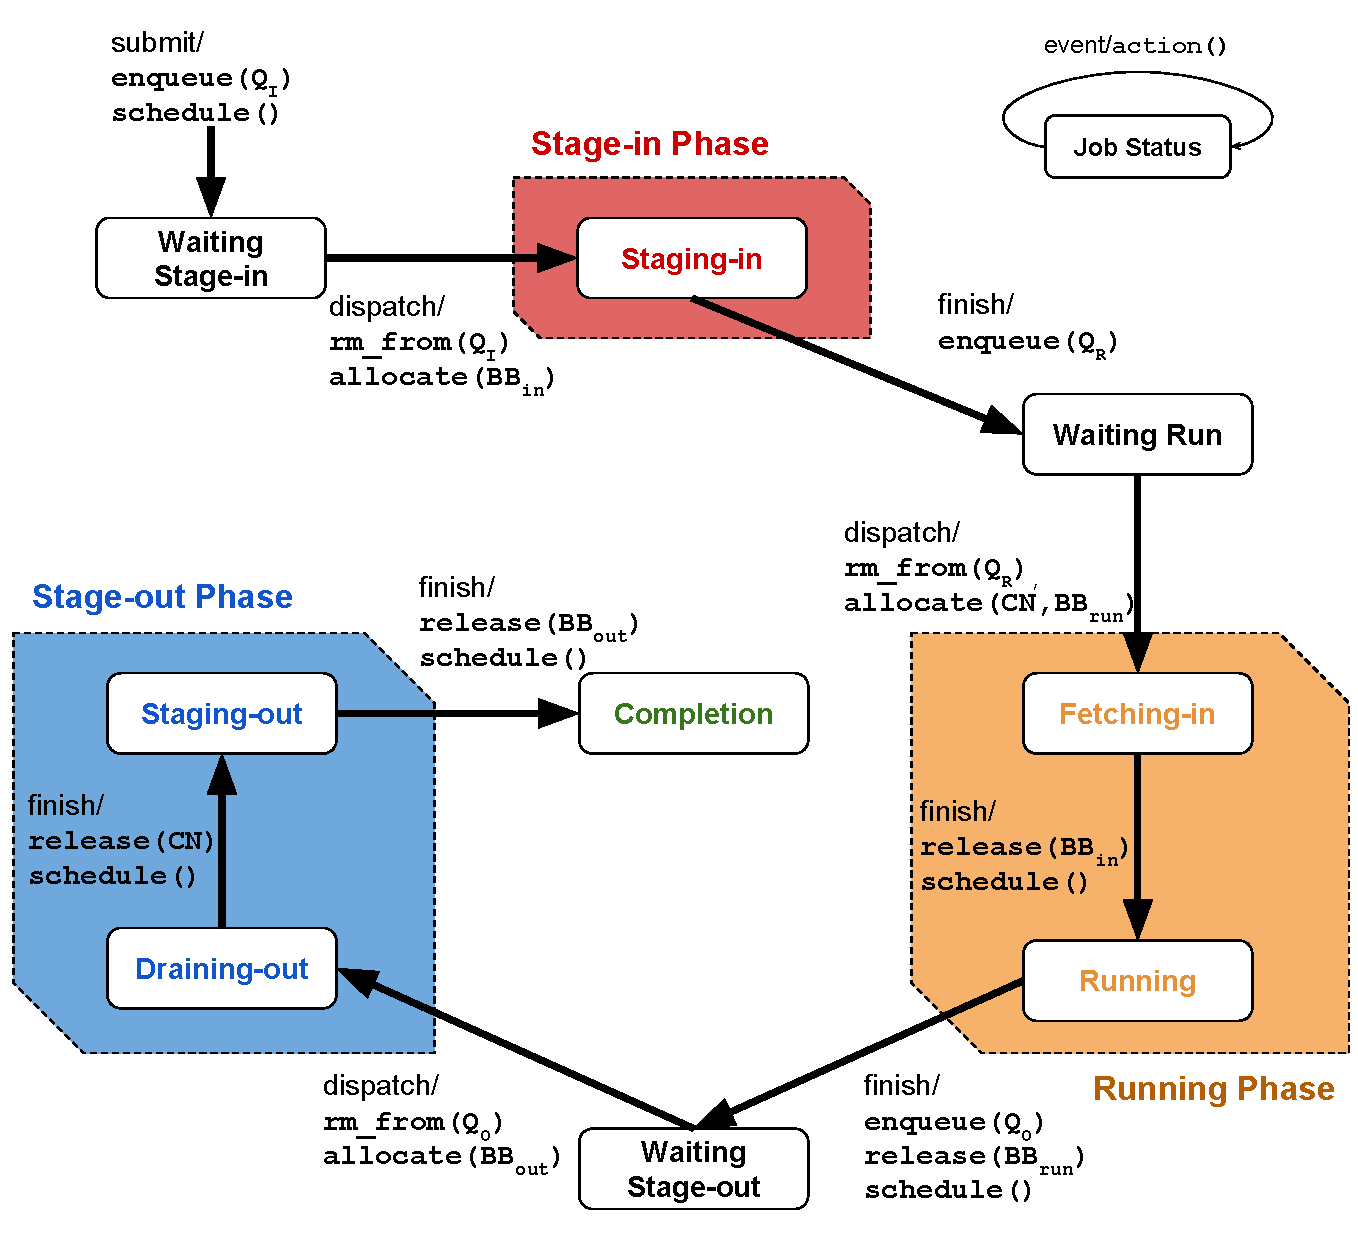
\includegraphics[width=3.6in]{3PhaseJobFSM}
%         \caption{Event-driven BBsim scheduling model}
% \label{Fig:JobFSM}
% \end{figure}
% 
% 
% Whenever $j_i$ enters one of the three phases, 
% system resources are allocated in the following way:
% \begin{itemize}
%         \item $BB_{in}$ TB amount of burst buffer are allocated upon entering stage-in phase.
%         \item $CN$ number of compute nodes and $BB_{run}$ amount of burst buffer
%                 are allocated upon entering running phase.
%         \item $BB_{out}$ TB of burst buffer are allocated upon entering stage-out phase.
% \end{itemize}
% Various \texttt{release()} actions are of importance because, in addition to submission,
% \texttt{schedule()} is invoked to schedule a waiting job. 
% The allocated resource can only be released when certain phase is finished. 
% Therefore, any \textit{dispatch} event, generated by \texttt{schedule()} action, 
% follows right after a certain \textit{finish} event.
% The allocated resources are released at the following time points:
% \begin{itemize}
%         \item When $j_i$ pre-fetched data is loaded from burst buffer to memory,
% %               burst buffer allocated in stage-in phase are released.
% 	      $BB_{in}$ is released.
%         \item When $j_i$ finishes computation, 
% % 	      system reclaims burst buffer allocated in running phase
% 	      $BB_{run}$ is released.
%         \item When $j_i$ output data is written to burst buffer from memory,
% %                 compute nodes allocated in running phase are released.
% 	      $CN$ is released.
%         \item When output data is drained out to external storage,
% %                 burst buffer allocated in stage-out phase are released. 
% 	      $BB_{out}$ is released.
%                 Job $j_i$ is completed and exits the system.
% \end{itemize}
% 
% 
% Though targeting on burst buffer enabled systems, 
% BBSim also supports simulating job scheduling on HPC systems without burst buffer.
% Besides, it is easy to integrate any scheduling policies into BBsim. 


